%%%%%%%%%%%%%%%%%%%%%%%%%%%%%%%%%%%%%%%%%
% Lachaise Assignment
% LaTeX Template
% Version 1.0 (26/6/2018)
%
% This template originates from:
% http://www.LaTeXTemplates.com
%
% Authors:
% Marion Lachaise & François Févotte
% Vel (vel@LaTeXTemplates.com)
%
% License:
% CC BY-NC-SA 3.0 (http://creativecommons.org/licenses/by-nc-sa/3.0/)
% 
%%%%%%%%%%%%%%%%%%%%%%%%%%%%%%%%%%%%%%%%%

%----------------------------------------------------------------------------------------
%	PACKAGES AND OTHER DOCUMENT CONFIGURATIONS
%----------------------------------------------------------------------------------------

\documentclass{article}
\usepackage{enumerate}
\usepackage{graphicx}
\usepackage{hyperref}
\usepackage{float}
%%%%%%%%%%%%%%%%%%%%%%%%%%%%%%%%%%%%%%%%%
% Lachaise Assignment
% Structure Specification File
% Version 1.0 (26/6/2018)
%
% This template originates from:
% http://www.LaTeXTemplates.com
%
% Authors:
% Marion Lachaise & François Févotte
% Vel (vel@LaTeXTemplates.com)
%
% License:
% CC BY-NC-SA 3.0 (http://creativecommons.org/licenses/by-nc-sa/3.0/)
% 
%%%%%%%%%%%%%%%%%%%%%%%%%%%%%%%%%%%%%%%%%

%----------------------------------------------------------------------------------------
%	PACKAGES AND OTHER DOCUMENT CONFIGURATIONS
%----------------------------------------------------------------------------------------

\usepackage{amsmath,amsfonts,stmaryrd,amssymb} % Math packages

\usepackage{enumerate} % Custom item numbers for enumerations

\usepackage[ruled]{algorithm2e} % Algorithms

\usepackage[framemethod=tikz]{mdframed} % Allows defining custom boxed/framed environments

\usepackage{listings} % File listings, with syntax highlighting
\lstset{
	basicstyle=\ttfamily, % Typeset listings in monospace font
}

%----------------------------------------------------------------------------------------
%	DOCUMENT MARGINS
%----------------------------------------------------------------------------------------

\usepackage{geometry} % Required for adjusting page dimensions and margins

\geometry{
	paper=a4paper, % Paper size, change to letterpaper for US letter size
	top=2.5cm, % Top margin
	bottom=3cm, % Bottom margin
	left=2.5cm, % Left margin
	right=2.5cm, % Right margin
	headheight=14pt, % Header height
	footskip=1.5cm, % Space from the bottom margin to the baseline of the footer
	headsep=1.2cm, % Space from the top margin to the baseline of the header
	%showframe, % Uncomment to show how the type block is set on the page
}

%----------------------------------------------------------------------------------------
%	FONTS
%----------------------------------------------------------------------------------------

\usepackage[utf8]{inputenc} % Required for inputting international characters
\usepackage[T1]{fontenc} % Output font encoding for international characters

\usepackage{XCharter} % Use the XCharter fonts

%----------------------------------------------------------------------------------------
%	COMMAND LINE ENVIRONMENT
%----------------------------------------------------------------------------------------

% Usage:
% \begin{commandline}
%	\begin{verbatim}
%		$ ls
%		
%		Applications	Desktop	...
%	\end{verbatim}
% \end{commandline}

\mdfdefinestyle{commandline}{
	leftmargin=10pt,
	rightmargin=10pt,
	innerleftmargin=15pt,
	middlelinecolor=black!50!white,
	middlelinewidth=2pt,
	frametitlerule=false,
	backgroundcolor=black!5!white,
	frametitle={Command Line},
	frametitlefont={\normalfont\sffamily\color{white}\hspace{-1em}},
	frametitlebackgroundcolor=black!50!white,
	nobreak,
}

% Define a custom environment for command-line snapshots
\newenvironment{commandline}{
	\medskip
	\begin{mdframed}[style=commandline]
}{
	\end{mdframed}
	\medskip
}

%----------------------------------------------------------------------------------------
%	FILE CONTENTS ENVIRONMENT
%----------------------------------------------------------------------------------------

% Usage:
% \begin{file}[optional filename, defaults to "File"]
%	File contents, for example, with a listings environment
% \end{file}

\mdfdefinestyle{file}{
	innertopmargin=1.6\baselineskip,
	innerbottommargin=0.8\baselineskip,
	topline=false, bottomline=false,
	leftline=false, rightline=false,
	leftmargin=2cm,
	rightmargin=2cm,
	singleextra={%
		\draw[fill=black!10!white](P)++(0,-1.2em)rectangle(P-|O);
		\node[anchor=north west]
		at(P-|O){\ttfamily\mdfilename};
		%
		\def\l{3em}
		\draw(O-|P)++(-\l,0)--++(\l,\l)--(P)--(P-|O)--(O)--cycle;
		\draw(O-|P)++(-\l,0)--++(0,\l)--++(\l,0);
	},
	nobreak,
}

% Define a custom environment for file contents
\newenvironment{file}[1][File]{ % Set the default filename to "File"
	\medskip
	\newcommand{\mdfilename}{#1}
	\begin{mdframed}[style=file]
}{
	\end{mdframed}
	\medskip
}

%----------------------------------------------------------------------------------------
%	NUMBERED QUESTIONS ENVIRONMENT
%----------------------------------------------------------------------------------------

% Usage:
% \begin{question}[optional title]
%	Question contents
% \end{question}

\mdfdefinestyle{question}{
	innertopmargin=1.2\baselineskip,
	innerbottommargin=0.8\baselineskip,
	roundcorner=5pt,
	nobreak,
	singleextra={%
		\draw(P-|O)node[xshift=1em,anchor=west,fill=white,draw,rounded corners=5pt]{%
		Question \theQuestion\questionTitle};
	},
}

\newcounter{Question} % Stores the current question number that gets iterated with each new question

% Define a custom environment for numbered questions
\newenvironment{question}[1][\unskip]{
	\bigskip
	\stepcounter{Question}
	\newcommand{\questionTitle}{~#1}
	\begin{mdframed}[style=question]
}{
	\end{mdframed}
	\medskip
}

%----------------------------------------------------------------------------------------
%	WARNING TEXT ENVIRONMENT
%----------------------------------------------------------------------------------------

% Usage:
% \begin{warn}[optional title, defaults to "Warning:"]
%	Contents
% \end{warn}

\mdfdefinestyle{warning}{
	topline=false, bottomline=false,
	leftline=false, rightline=false,
	nobreak,
	singleextra={%
		\draw(P-|O)++(-0.5em,0)node(tmp1){};
		\draw(P-|O)++(0.5em,0)node(tmp2){};
		\fill[black,rotate around={45:(P-|O)}](tmp1)rectangle(tmp2);
		\node at(P-|O){\color{white}\scriptsize\bf !};
		\draw[very thick](P-|O)++(0,-1em)--(O);%--(O-|P);
	}
}

% Define a custom environment for warning text
\newenvironment{warn}[1][Warning:]{ % Set the default warning to "Warning:"
	\medskip
	\begin{mdframed}[style=warning]
		\noindent{\textbf{#1}}
}{
	\end{mdframed}
}

%----------------------------------------------------------------------------------------
%	INFORMATION ENVIRONMENT
%----------------------------------------------------------------------------------------

% Usage:
% \begin{info}[optional title, defaults to "Info:"]
% 	contents
% 	\end{info}

\mdfdefinestyle{info}{%
	topline=false, bottomline=false,
	leftline=false, rightline=false,
	nobreak,
	singleextra={%
		\fill[black](P-|O)circle[radius=0.4em];
		\node at(P-|O){\color{white}\scriptsize\bf i};
		\draw[very thick](P-|O)++(0,-0.8em)--(O);%--(O-|P);
	}
}

% Define a custom environment for information
\newenvironment{info}[1][Info:]{ % Set the default title to "Info:"
	\medskip
	\begin{mdframed}[style=info]
		\noindent{\textbf{#1}}
}{
	\end{mdframed}
}
 % Include the file specifying the document structure and custom commands
\usepackage{listings}

%----------------------------------------------------------------------------------------
%	ASSIGNMENT INFORMATION
%----------------------------------------------------------------------------------------

\title{EBD13 Gerência de Dados e Computação em Nuvem} % Title of the assignment

\author{Alexandre Miyazaki\\ \texttt{aksmiyazaki@gmail.com}} % Author name and email address

\date{Universidade Federal do Rio Grande do Sul} % University, school and/or department name(s) and a date

%----------------------------------------------------------------------------------------

\begin{document}

\maketitle % Print the title

\section*{Objetivo do Trabalho} % Unnumbered section

O objetivo do trabalho era:

\begin{itemize}
\item Criar uma infraestrutura computacional em nuvem;
\item Realizar o deploy de um ambiente que seja capaz de analisar dados nesse ambiente;
\item Realizar uma análise simples.
\end{itemize}

Nas próximas seções estão os passos para atingir tais objetivos.


\section{Criando Infraestrutura} % Numbered section

Para criação da infraestrutura, foi escolhida a AWS, pois foi o ambiente no qual o professor realizou o laboratório.

\begin{figure}[H]
  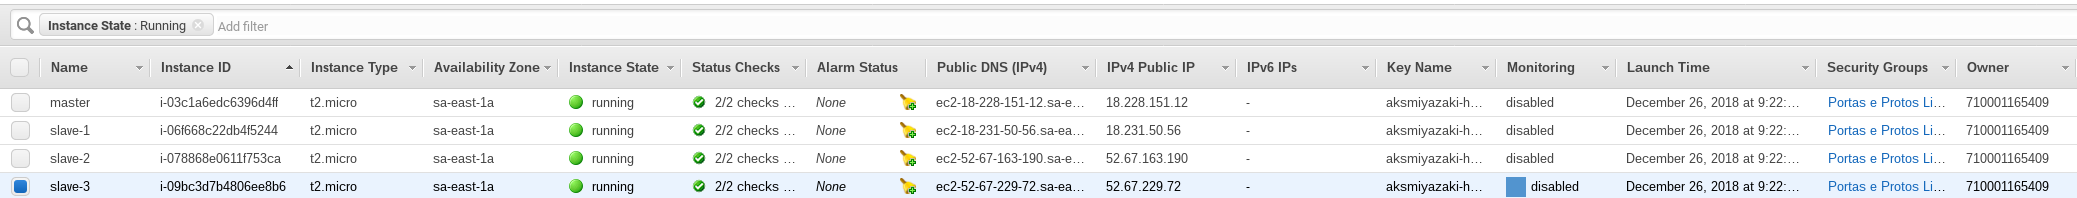
\includegraphics[width=\linewidth]{img/machines_created.png}
  \caption{Máquinas criadas na \emph{cloud}.}
  \label{fig:fig_maq_criad}
\end{figure}

A Figura \ref{fig:fig_maq_criad} mostra a infraestrutura de máquinas. Foram criados 4 nós na AWS, sendo um deles o Mestre e os demais, escravos. 
A parte de segurança da rede na própria AWS foi negligenciada, deixando todas as portas abertas. Abaixo, a Figura \ref{fig:machine_config} mostra parte da configuração das máquinas na AWS.


\begin{figure}[H]
  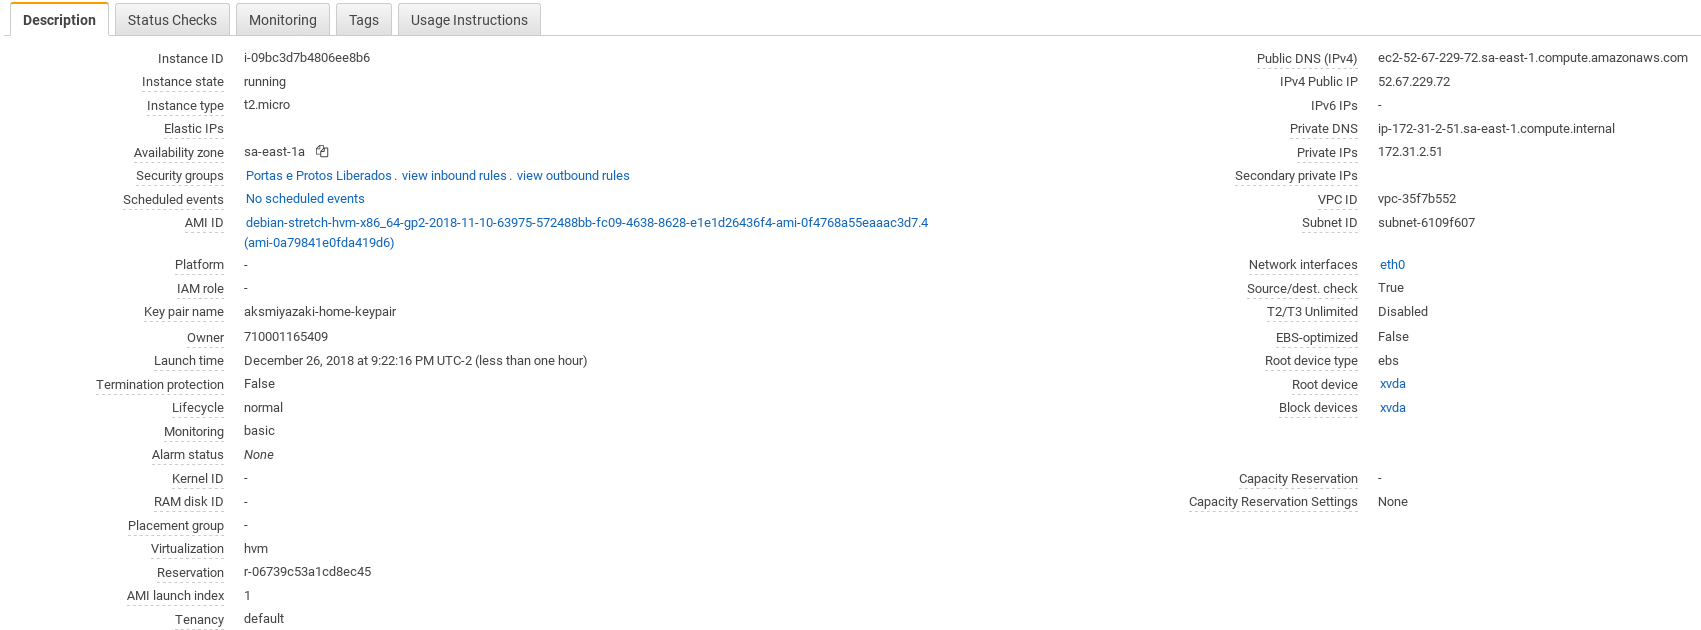
\includegraphics[width=\linewidth]{img/machine_config.png}
  \caption{Parte da configuração dos nós.}
  \label{fig:machine_config}
\end{figure}

Antes de passarmos para a próxima Seção, precisamos conseguir acessar as máquinas criadas. O trabalho foi realizado
em uma máquina Linux, de forma que isso se torna fácil via ssh. A Figura \ref{fig:machine_access} mostra o processo para acessar a máquina via terminal.

\begin{figure}[H]
  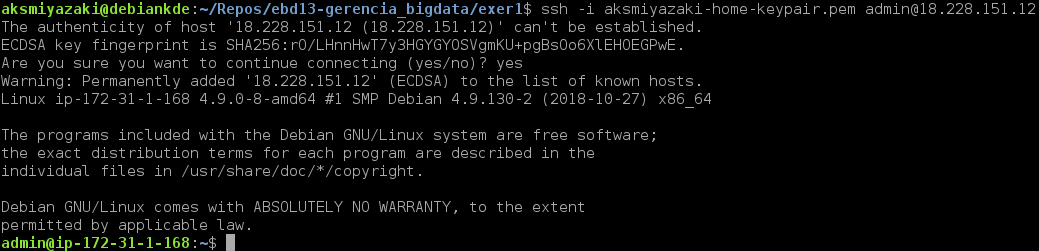
\includegraphics[width=\linewidth]{img/machine_access.png}
  \caption{Acesso aos nós via ssh.}
  \label{fig:machine_access}
\end{figure}

\newpage
\section{Deploy de Ambiente}

Iniciando o deploy do ambiente, foram instalados os pacotes requisitados. A Figura \ref{fig:package_install} exibe a linha de comando executada
para a instalação dos pacotes. Essa linha de comando foi executada em todos os nós (Master e 3 Slaves).

\begin{figure}[H]
  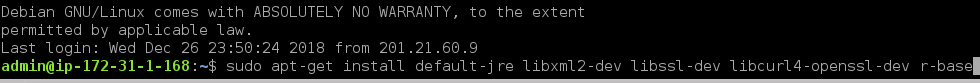
\includegraphics[width=\linewidth]{img/package_install.png}
  \caption{Linha de comando executada para instalação de pacotes.}
  \label{fig:package_install}
\end{figure}

Após esse processo, o Hadoop deve ser baixado e instalado nas máquinas. O comando exibido na Figura \ref{fig:hadoop_dl} foi executado em todos os nós da arquitetura.
Com o sistema baixado e descompactado, o ambiente está ok para continuarmos.

\begin{figure}[H]
  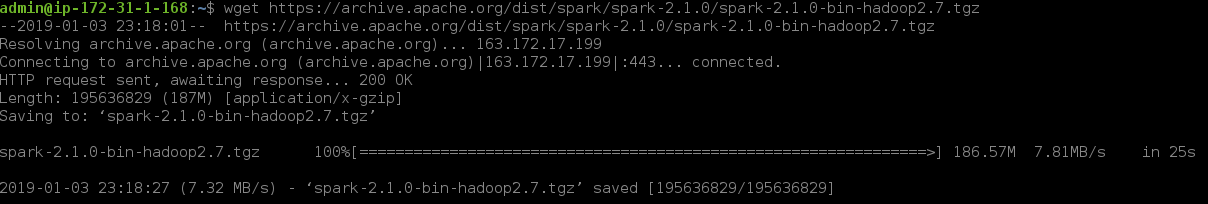
\includegraphics[width=\linewidth]{img/hadoop_download.png}
  \caption{Download do Hadoop.}
  \label{fig:hadoop_dl}
\end{figure}

\subsection{Executando o Spark no Ambiente}

Após a configuração, está na hora de executarmos o Master. Para isso, antes é necessário setar algumas variáveis de ambiente:


\begin{itemize}
\item SPARK\_LOCAL\_IP: é o IP onde da máquina vinculada ao Spark;
\item SPARK\_MASTER\_HOST: é o IP onde está rodando o nó Mestre.
\end{itemize}

Realizadas essas configurações, pode-se executar o Master com o script \emph{start-master.sh}. Ele gera um log ao executar, mostrado na Figura \ref{fig:spark_log}.

\begin{figure}[h]
  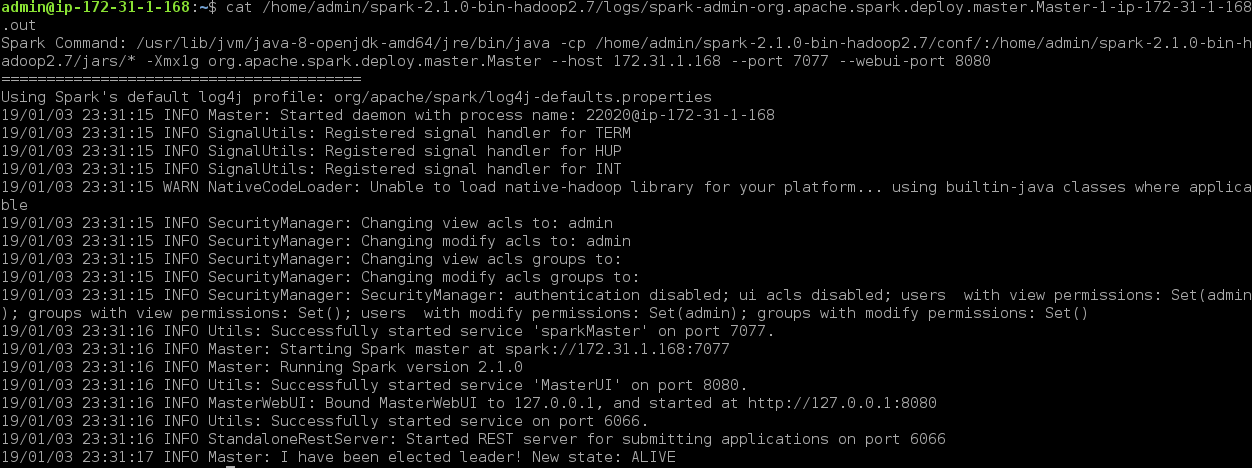
\includegraphics[width=\linewidth]{img/spark_log.png}
  \caption{Log do nó Master inicializado.}
  \label{fig:spark_log}
\end{figure}

Agora, vamos inicializar as instâncias dos Slaves. Para isso, precisamos executar o script \emph{start-slave.sh}, parametrizando o endereço do Master com a porta.
Realizado esse processo, o log do próprio Master acusa que os nós foram conectados, como mostra a Figura \ref{fig:env_ready}.

\begin{figure}[h]
  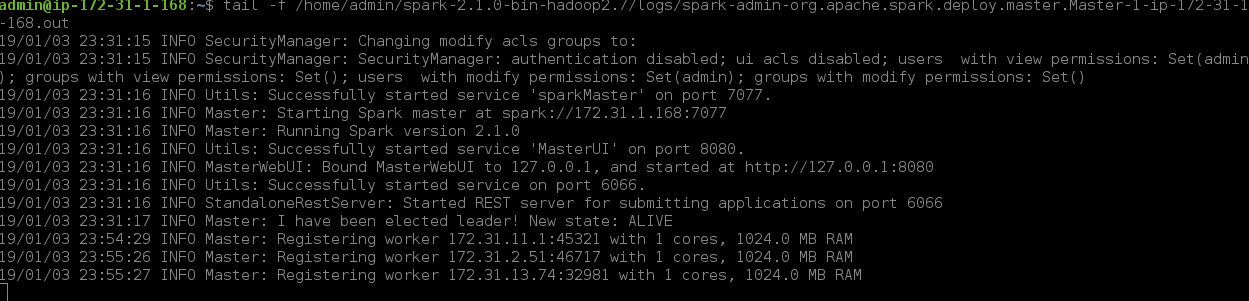
\includegraphics[width=\linewidth]{img/environment_ready.png}
  \caption{Mestre com os Slaves conectados.}
  \label{fig:env_ready}
\end{figure}

\subsection{Fazendo o Deploy do Jupyter}

Neste trabalho, decidi por utilizar Python e PySpark (já como uma preparação para o trabalho final). Para isso, realizei o Deploy do Jupyter.

Inicialmente, baixei e instalei o \href{https://www.anaconda.com/download/#linux}{Anaconda} todavia, por algum motivo, o Python ainda era reconhecido como o que já vem instalado no sistema. Ao dar um reboot na máquina, ele reconheceu o certo (e posteriormente, achei uma forma mais simples de fazer, usando o comando \empth{source .bashrc}, pois o Anaconda faz mudanças no arquivo .bashrc).

Feito isso, foram executados uma série de comandos e edição de arquivos de configuração para subir o Jupyter, eles podem ser visualizados \href{https://medium.com/@josemarcialportilla/getting-spark-python-and-jupyter-notebook-running-on-amazon-ec2-dec599e1c297}{neste link}. Acredito que fuja do escopo do trabalho detalhar essa parte, portanto fica o tutorial como registro.

Após a realização das configurações (vale salientar que uma delas é configuração de senha, e que o setup dele na Amazon foi menos \emph{plug-and-play} do que setar localmente), foi possível acessar o Jupyter remotamente, conforme mostra a Figura \ref{fig:acess_jupyter}.

\begin{figure}[H]
  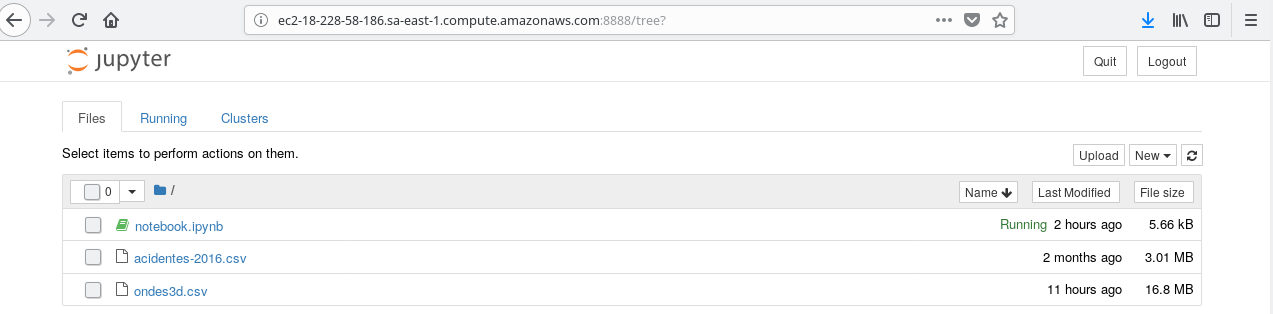
\includegraphics[width=\linewidth]{img/jupyter_access.png}
  \caption{Acesso ao Jupyter Notebook.}
  \label{fig:acess_jupyter}
\end{figure}

\subsection{Configurando o PySpark}

Para rodar o Spark com Python, é necessário instalar a biblioteca Pyspark, além de declarar algumas variáveis de ambiente. Inicialmente, instalou-se o PySpark (Figura \ref{fig:pyspark_install}).

\begin{figure}[H]
  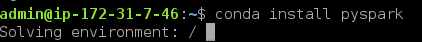
\includegraphics[width=\linewidth]{img/install_pyspark.png}
  \caption{Instalação do Pyspark.}
  \label{fig:pyspark_install}
\end{figure}

Após realizar essa instalação, as seguintes variáveis de ambiente foram configuradas:

\begin{itemize}
    \item export SPARK\_HOME='/home/admin/spark-2.1.0-bin-hadoop2.7'
    \item export PATH=\$SPARK\_HOME:\$PATH
    \item export PYTHONPATH=\$SPARK\_HOME/python:\$PYTHONPATH
\end{itemize}

Agora, partimos para a parte de carregar os dados e analisá-los.


\newpage
\section{Análise de dados}

Decidiu-se por fazer uma análise superficial, tendo em vista que o escopo do trabalho era mais focado em montar o ambiente. Para isso, utilizou-se o arquivo de acidentes de 2016, disponibilizado pelo professor. Para começar, criamos uma SparkSession e lemos o dataframe do arquivo, conforme mostrado abaixo.

\begin{lstlisting}[language=Python]
spark = SparkSession.builder \
   .master("local") \
   .appName("EBD13-EXER") \
   .config("spark.executor.memory", "800mb") \
   .getOrCreate()
   
sc = spark.sparkContext
sqlContext = SQLContext(sc)

df = sqlContext.read.option("delimiter", ';')
.load('file:///home/admin/Notebooks/acidentes-2016.csv', 
                      format='com.databricks.spark.csv', 
                      header='true', 
                      inferSchema='true')
\end{lstlisting}

Com isso, conseguimos carregar os dados na conexão, abaixo uma parte da descrição do esquema desses dados (Figura \ref{fig:df_description}).

\begin{figure}[H]
  \centering
  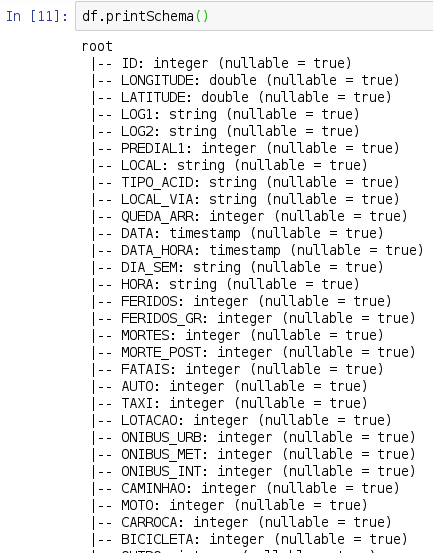
\includegraphics[width=0.5 \linewidth]{img/df_description.png}
  \caption{Descrição dos dados.}
  \label{fig:df_description}
\end{figure}

Após, utilizamos o código abaixo para criar uma tabela dentro do framework. Agora podemos utilizar SQL para consultá-la (via Spark).

\begin{lstlisting}[language=Python]
df.createOrReplaceTempView("table_acidentes")
\end{lstlisting}

Consultando uma informação simples nos dados, identificamos que há 47 mortos no ano (Figura \ref{fig:df_dead_no}). Na primeira análise, irei verificar a distribuição de mortes por dia da semana.

\begin{figure}[H]
  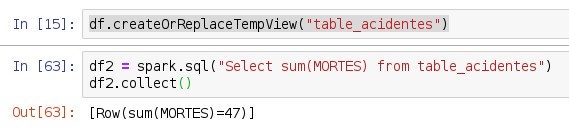
\includegraphics[width=\linewidth]{img/df_numberofdead.png}
  \caption{Consulta simples na tabela criada.}
  \label{fig:df_dead_no}
\end{figure}

Para manipular os dados localmente (no \emph{frontend} Python), utilizei o pacote Pandas. Além dele, utilizei o Seaborn e o Matplotlib para plotar os dados. Fazendo a consulta agrupando pelo campo \textbf{DIA\_SEM}, e plotando os dados, o gráfico gerado pode ser visualizado na Figura \ref{fig:df_dead_by_week}. O dia em que mais houve mortes foi sábado, o que faz sentido tendo em vista que é final de semana. Todavia, esse não parece um resultado convincente, portanto, vamos analisar a distribuição de todos os acidentes.

\begin{figure}[H]
  \centering
  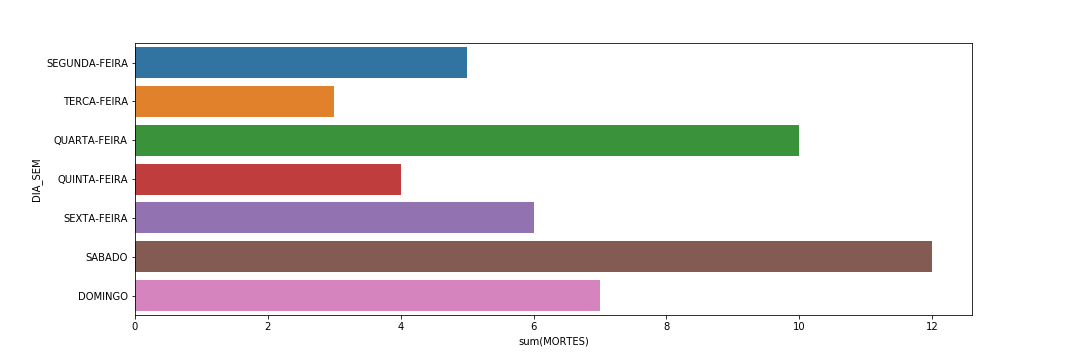
\includegraphics[width=\linewidth]{img/dead_by_week.png}
  \caption{Plot de mortes, agrupado por dia da semana.}
  \label{fig:df_dead_by_week}
\end{figure}


Conforme a Figura \ref{fig:acid_by_weekday} mostra, o número de acidentes cai no Sábado e Domingo. Isso pode indicar que, apesar de ter menos acidentes no final de semana, eles acabam sendo mais fatais.

\begin{figure}[H]
  \centering
  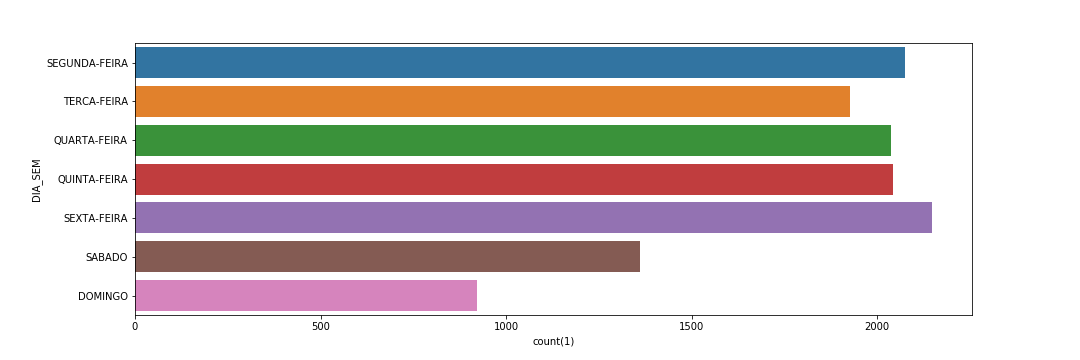
\includegraphics[width=\linewidth]{img/acid_by_weekday.png}
  \caption{Acidentes por dia de semana.}
  \label{fig:acid_by_weekday}
\end{figure}

Feito isso, decidi por analisar os tipos mais frequentes de acidentes. Para isso, outra consulta foi realizada, o resultado está ilustrado na Figura \ref{fig:df_acid_type}. A distribuição de acidentes faz sentido, tendo em vista que é comum ver uma Colisão ou um Abalroamento (tipo de batida também), e os menos comuns são aqueles que dificilmente vemos, como Capotagem e Incêndio.

\begin{figure}[H]
  \centering
  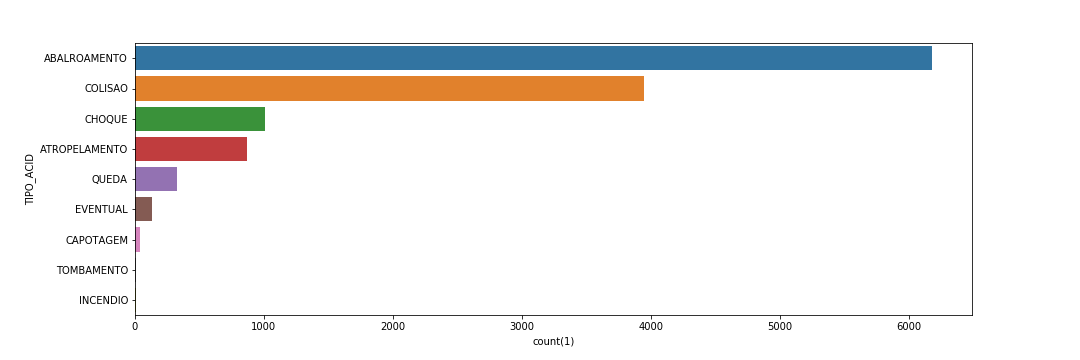
\includegraphics[width=\linewidth]{img/tipo_acid.png}
  \caption{Plot de acidentes por tipo.}
  \label{fig:df_acid_type}
\end{figure}

\section{Considerações Finais}

O trabalho foi muito interessante, fazia algum tempo que eu não montava um ambiente distribuído a mão. Houveram algumas dificuldades, principalmente pois nunca tinha feito o Deploy do Jupyter para utilizar remoto e nem utilizado o PySpark. Todavia, após superar essas dificuldades pontuais, tudo correu bem.

Tendo em vista que o objetivo do trabalho era mais para criar e utilizar o ambiente, decidi por fazer uma análise de dados bem superficial, apenas para ilustrar o uso do ambiente. Facilmente poderia aprofundar essas análises, contudo, acho mais interessante fazer análises mais rebuscadas no trabalho final da disciplina.

\end{document}